\chapter{Results}

In this chapter we will show the results obtained in this work. They will be divided between the three metrics we chose to monitor (see section Experiment Design in the Development chapter).

\section{Rasterization Baseline}
First of all and as a sanity check, we will compare the performance of a renderer using ray tracing to one drawing the same geometry through rasterization. The model chosen for this will be the Viking Room from the Vulkan Tutorial \cite{VulkanTutorial}.

In the first place we will look at how video memory usage changes as the frame sizes get bigger. We can see a comparison of how much memory both renderers employ in graph \ref{memory-usage-comparison-graph}. We see an expected increase in memory consumption as the frame buffer resolutions get bigger, as well as a huge difference, of about an order of magnitude, between the two methods for any given resolution. This is to be expected not only because a bigger frame buffer will require more memory to be stored, but also because the ray tracer requires to store an acceleration structure as well as all the possible shaders bound at the same time.


\begin{figure}[hbt!]
    \centering
    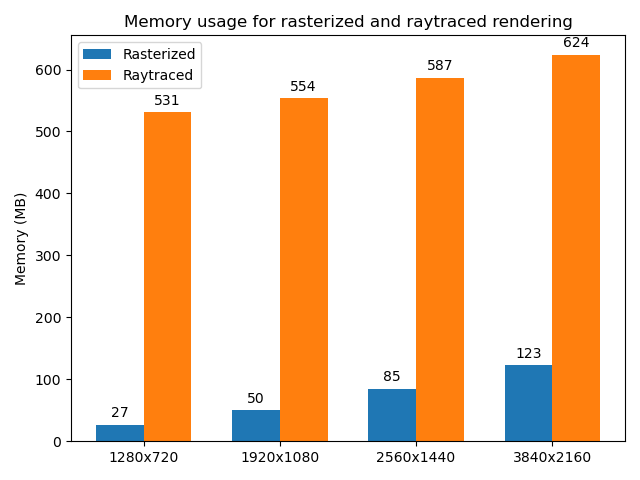
\includegraphics[width=1.0\textwidth]{figuras/vulkan-memory-usage-comparison.png}
    \caption{GPU memory consumption when rendering the Viking Room 3D model at a range of reasonable resolutions, using ray traced and traditionally rasterized graphics. We can see a significant difference between the two, as well as an expected increase as resolutions get higher.}
    \label{memory-usage-comparison-graph}
\end{figure}
\section{Memory Usage}
\section{Acceleration Structure Build Time}
\section{Frame Time}
